\begin{frame}{Definitions}
    \begin{block}{Un tableau}
        En programmation,
        on parle de tableau pour d\'esigner un \textbf{ensemble d'\'el\'ements} de m\^eme type design\'e par un nom unique,
        chaque \'el\'ement \'etant rep\'er\'e par un \textbf{indice} pr\'ecisant sa position au sein de l'ensemble
    \end{block}
    \center{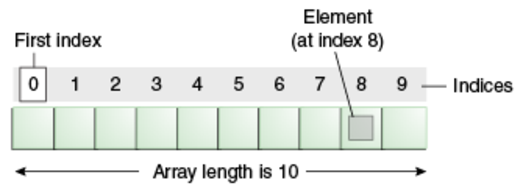
\includegraphics[height=4em]{images/objects-tenElementArray}}
\end{frame}